\section{Integration von Dependency Scanning und Überprüfung auf Sicherheitslücken in den DevOps-Zyklus}
In diesem Kapitel wird anhand von Dependency Scanning und der Überprüfung auf Sicherheitslücken aufgezeigt, wie Sicherheitslücken in Abhängigkeiten erkannt und behoben werden können, bevor diese in für den Produktionsbetrieb freigegebenen Releases veröffentlicht und in Betrieb genommen werden.

\subsection{Nutzung von Dependency Scanning}
Dependency Scanning und die Überprüfung auf Sicherheitslücken sind kritische Schritte im Softwareentwicklungsprozess, um sicherzustellen, dass alle verwendeten Bibliotheken und Abhängigkeiten sicher und auf dem neuesten Stand sind. Es gibt mehrere Tools, die für diesen Zweck verwendet werden können, darunter Sonatype Nexus IQ, Snyk und OWASP Dependency-Check. Die Autoren dieses Kapitels fokussieren sich auf die Verwendung von Sonatype Nexus IQ aufgrund ihrer umfassenden Erfahrung und der weitreichenden Fähigkeiten dieses Tools.

\subsubsection{Übersicht ähnlicher Produkte}

Es gibt verschiedene Tools, die zur Überprüfung von Abhängigkeiten auf Sicherheitslücken verwendet werden können. Die folgende Tabelle gibt eine Übersicht über einige gängige Tools:

\begin{table*}[h!]
\centering
\begin{tabular}{|l|l|l|l|}
\hline
\textbf{Tool} & \textbf{Programmiersprachen} & \textbf{Lizenz} & \textbf{Besonderheiten} \\ \hline
Sonatype Nexus IQ & Mehrere & Proprietär & Umfassende Sicherheitsanalyse, Policy Enforcement \\ \hline
Snyk & Mehrere & Proprietär & Echtzeit-Schwachstellenüberprüfung, Entwicklungsintegration \\ \hline
OWASP Dependency-Check & Mehrere & Open Source & Fokus auf bekannte Sicherheitslücken \\ \hline
WhiteSource & Mehrere & Proprietär & Automatisierte Open-Source-Sicherheit und Compliance \\ \hline
Black Duck & Mehrere & Proprietär & Umfassende Open-Source-Risikoanalyse \\ \hline
\end{tabular}
\caption{Übersicht von Tools zur Überprüfung von Abhängigkeiten}
\label{tab:dependency_scanning_tools}
\end{table*}

\subsubsection{Funktionsweise von Sonatype Nexus IQ}

Sonatype Nexus IQ ist ein fortschrittliches Tool zur Analyse von Abhängigkeiten und zur Erkennung von Sicherheitslücken. Es arbeitet durch:

\begin{itemize}
    \item \textbf{Scannen der Abhängigkeiten}: Analysiert alle im Projekt verwendeten Abhängigkeiten.
    \item \textbf{Abgleich mit Datenbanken}: Vergleicht Abhängigkeiten mit bekannten Schwachstellen in öffentlichen und privaten Datenbanken.
    \item \textbf{Policy Enforcement}: Überprüft Abhängigkeiten gegen vordefinierte Sicherheitsrichtlinien und Policies.
    \item \textbf{Berichterstellung}: Generiert Berichte und Warnungen über erkannte Sicherheitslücken und Risiken.
\end{itemize}

\begin{figure*}[h!]
\centering
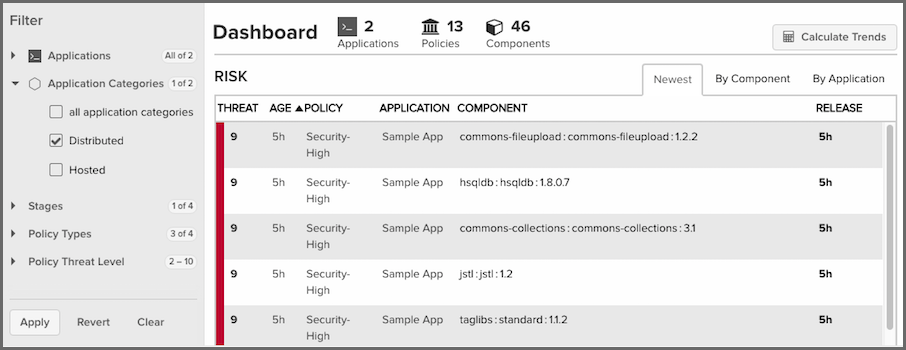
\includegraphics[width=\textwidth]{nexusiq_dashboard.png}
\caption{Beispiel eines Sonatype Nexus IQ Dashboards}
\label{fig:nexusiq_dashboard}
\end{figure*}

\subsubsection{Vorteile von Sonatype Nexus IQ}

Die Verwendung von Sonatype Nexus IQ bietet zahlreiche Vorteile:

\begin{itemize}
    \item \textbf{Umfassende Sicherheitsanalyse}: Erkennt eine Vielzahl von Schwachstellen in Abhängigkeiten.
    \item \textbf{Automatisierte Policy Enforcement}: Stellt sicher, dass nur sichere und konforme Abhängigkeiten verwendet werden.
    \item \textbf{Integration in CI/CD}: Kann nahtlos in bestehende CI/CD-Pipelines integriert werden.
    \item \textbf{Detaillierte Berichte}: Bietet umfangreiche Berichte und Dashboards zur Überwachung der Sicherheit.
    \item \textbf{Regelmäßige Updates}: Erhält kontinuierliche Updates zu neuen Sicherheitslücken und Bedrohungen.
\end{itemize}

\subsubsection{Beispiel Implementierung für GitHub Actions}

Ein typisches Setup für die Integration von Sonatype Nexus IQ in GitHub Actions könnte wie folgt aussehen:

\paragraph{Einrichtung der GitHub Actions Workflow-Datei}

Erstellen Sie im Wurzelverzeichnis Ihres Repositories eine Datei namens \texttt{.github/workflows/nexus-iq.yml} mit folgendem Inhalt:

\begin{lstlisting}
name: Nexus IQ Analysis

on:
  push:
    branches:
      - main
      - develop
  pull_request:
    branches:
      - main
      - develop

jobs:
  nexusIQ:
    runs-on: ubuntu-latest

    steps:
    - name: Check out repository
      uses: actions/checkout@v2

    - name: Set up JDK 11
      uses: actions/setup-java@v1
      with:
        java-version: '11'

    - name: Cache Nexus IQ packages
      uses: actions/cache@v2
      with:
        path: ~/.nexus/cache
        key: ${{ runner.os }}-nexus-cache
        restore-keys: ${{ runner.os }}-nexus-cache

    - name: Install dependencies
      run: ./gradlew build -x test

    - name: Run Nexus IQ analysis
      env:
        NEXUS_IQ_URL: ${{ secrets.NEXUS_IQ_URL }}
        NEXUS_IQ_USERNAME: ${{ secrets.NEXUS_IQ_USERNAME }}
        NEXUS_IQ_PASSWORD: ${{ secrets.NEXUS_IQ_PASSWORD }}
      run: ./gradlew nexusIqScan -Dsonar.projectKey=my_project_key -Dsonar.host.url=${{ secrets.NEXUS_IQ_URL }} -Dsonar.login=${{ secrets.NEXUS_IQ_USERNAME }} -Dsonar.password=${{ secrets.NEXUS_IQ_PASSWORD }}
\end{lstlisting}

\subsubsection{Integration in den GitFlow}

Die Integration von Dependency Scanning in den GitFlow-Prozess folgt einem ähnlichen Muster wie bei der statischen Code Analyse:

\begin{itemize}
    \item \textbf{Feature-Branches}: Scannen der Abhängigkeiten während der Entwicklung neuer Features.
    \item \textbf{Develop-Branch}: Regelmäßiges Scannen vor dem Mergen von Feature-Branches.
    \item \textbf{Release-Branches}: Finales Scannen vor der Freigabe neuer Releases.
    \item \textbf{Hotfix-Branches}: Schnelles Scannen bei dringenden Fehlerbehebungen.
\end{itemize}

\paragraph{Beispielhafte Umsetzung in GitHub}

\begin{enumerate}
    \item Forke das Repository und erstelle einen neuen Branch: \texttt{git checkout -b feature/new-feature develop}
    \item Implementiere das neue Feature und pushe die Änderungen: \texttt{git push origin feature/new-feature}
    \item Öffne einen Pull Request von \texttt{feature/new-feature} nach \texttt{develop}.
    \item Die CI/CD-Pipeline führt das Dependency Scanning mit Sonatype Nexus IQ durch.
    \item Bestehen alle Checks, kann der Branch gemerged werden.
\end{enumerate}

\subsubsection{Sicherheitsgewinn durch Dependency Scanning}

Die Integration von Dependency Scanning und der Überprüfung auf Sicherheitslücken in den CI/CD-Prozess bietet erhebliche Sicherheitsvorteile:

\begin{itemize}
    \item \textbf{Früherkennung von Sicherheitslücken}: Sicherheitslücken in Abhängigkeiten werden frühzeitig erkannt und können behoben werden, bevor sie in die Produktionsumgebung gelangen.
    \item \textbf{Kontinuierliche Überwachung}: Durch kontinuierliches Scannen werden neue Schwachstellen sofort erkannt.
    \item \textbf{Compliance und Sicherheit}: Durchsetzen von Sicherheitsrichtlinien und Compliance-Anforderungen.
\end{itemize}

\subsubsection{Warnhinweise und Einschränkungen}

Es ist wichtig zu beachten, dass trotz der Verwendung von Tools wie Sonatype Nexus IQ Sicherheitslücken in Abhängigkeiten dennoch vorhanden sein können. Entwickler sollten sich dessen bewusst sein und folgende Vorsichtsmaßnahmen treffen:

\begin{itemize}
    \item \textbf{Regelmäßige Updates}: Stellen Sie sicher, dass alle Abhängigkeiten regelmäßig auf die neuesten Versionen aktualisiert werden.
    \item \textbf{Manuelle Überprüfungen}: Ergänzen Sie automatisierte Scans durch manuelle Überprüfungen und Sicherheitsaudits.
    \item \textbf{Bewusstsein und Schulung}: Schulen Sie das Entwicklungsteam in Best Practices der sicheren Softwareentwicklung.
    \item \textbf{Kontinuierliche Verbesserung}: Passen Sie Sicherheitsrichtlinien und -prozesse kontinuierlich an neue Bedrohungen und Schwachstellen an.
\end{itemize}

\subsubsection{Details zu OWASP}

Die Open Web Application Security Project (OWASP) bietet eine Vielzahl von Ressourcen zur Verbesserung der Software-Sicherheit. Das OWASP Top Ten Projekt ist eine jährlich aktualisierte Liste der am häufigsten auftretenden und kritischsten Sicherheitsrisiken für Webanwendungen. Einige der in Sonatype Nexus IQ integrierten OWASP-Regeln umfassen:

\begin{itemize}
    \item \textbf{Injection}: Schutz vor verschiedenen Injektionstypen, einschließlich SQL-Injection.
    \item \textbf{Broken Authentication}: Überprüfung auf Schwachstellen in der Authentifizierung.
    \item \textbf{Sensitive Data Exposure}: Sicherstellung der Verschlüsselung sensibler Daten.
    \item \textbf{XML External Entities (XXE)}: Erkennung von Schwachstellen, die durch externe XML-Entitäten verursacht werden.
    \item \textbf{Broken Access Control}: Verhinderung von unbefugtem Zugriff auf Ressourcen.
\end{itemize}

\subsubsection{Schlussfolgerungen und Best Practices}

Die Integration von Dependency Scanning in den CI/CD-Prozess verbessert nicht nur die Sicherheit der Software, sondern trägt auch zur Einhaltung von Compliance-Richtlinien bei. Tools wie Sonatype Nexus IQ bieten umfassende Analysen und automatisierte Policy Enforcement, um Sicherheitslücken frühzeitig zu erkennen und zu beheben. Es ist jedoch entscheidend, Sicherheitsmaßnahmen kontinuierlich zu überwachen und anzupassen, um den höchsten Sicherheitsstandard zu gewährleisten.